\documentclass{scrartcl}
\usepackage[mathletters]{ucs}
\usepackage[utf8x]{inputenc}
\usepackage{amssymb}
\usepackage{amsmath}
\usepackage[usenames]{color}
\usepackage{hyperref}
\usepackage{wasysym}
\usepackage{graphicx}
\usepackage[normalem]{ulem}
\usepackage{enumerate}

\usepackage{listings}

\lstset{ %
basicstyle=\footnotesize,       % the size of the fonts that are used for the code
showspaces=false,               % show spaces adding particular underscores
showstringspaces=false,         % underline spaces within strings
showtabs=false,                 % show tabs within strings adding particular underscores
frame=single,                   % adds a frame around the code
tabsize=2,                      % sets default tabsize to 2 spaces
breaklines=true,                % sets automatic line breaking
breakatwhitespace=false,        % sets if automatic breaks should only happen at whitespace
}


\title{Masterproef Tool Wear Inspection - Update 4 DH}
\date{dinsdag 08 december 2020}
\author{}

\begin{document}

\maketitle

		\section{Masterproef Tool Wear Inspection - Update 4 DH}

Created vrijdag 20 november 2020



\subsection{Mail}

Beste meneer Hulens,

 

Ik heb intussen de problemen kunnen oplossen met de trage communicatie tussen de Arduino en de computer: de Arduino bleef 1 seconde wachten op een serial input signaal waardoor er heel veel vertraging optrad. De vertraging is nu teruggebracht tot +-1 miliseconde.

 

Echter heb ik een ander probleem, de houder die bij de camera was geleverd is onvoldoende. Deze kan niet goed genoeg vast gezet worden waardoor deze beweegt bij elke aanpassing van de setup of bij het scherpstellen van de lens. En het is hier niet makkelijk om een positie in te stellen en daar de positie van op te slaan om nadien een zelfde camera opstelling terug te kunnen maken. Liefst zou ik iets hebben waarbij de hoeken en de hoogte van de camera afleesbaar zijn of toch op een manier kwantiseerbaar.

 

Zijn er houders voorhanden op de campus? Ik denk hierbij bijvoorbeeld aan een houder van de proefbuizen van chemie?

 

Met vriendelijke groeten,

 

Lars De Pauw



\subsection{Mail}

Beste meneer Hulens,

 

Ik heb een nieuwe draaischijf geprint die de plaatjes wat beter kan vastzetten waardoor deze niet meer verschuiven en het iets makkelijker aanpasbaar is zonder het hele rad opnieuw te hoeven printen. Dit door de plaatjes vast te zetten met een clipje dat apart kan geprint worden (te zien op de foto in bijlage). Echter merk ik hier dat deze snel afbreken. Ik denk dat als ik dezelfde clipjes kan 3D printen met ABS in plaats van PLA het een stuk steviger zou worden. Dan kunnen de clipjes ook meteen in zwarte ABS geprint worden om geen licht weerkaatsing te hebben.

Ikzelf heb enkel witte PLA, moet ik dan zelf ABS bestellen of kan dat via u besteld worden? Het gaat maar over ongeveer 50 gram dus een overschot van ergens zal misschien ook al voldoende zijn.

 

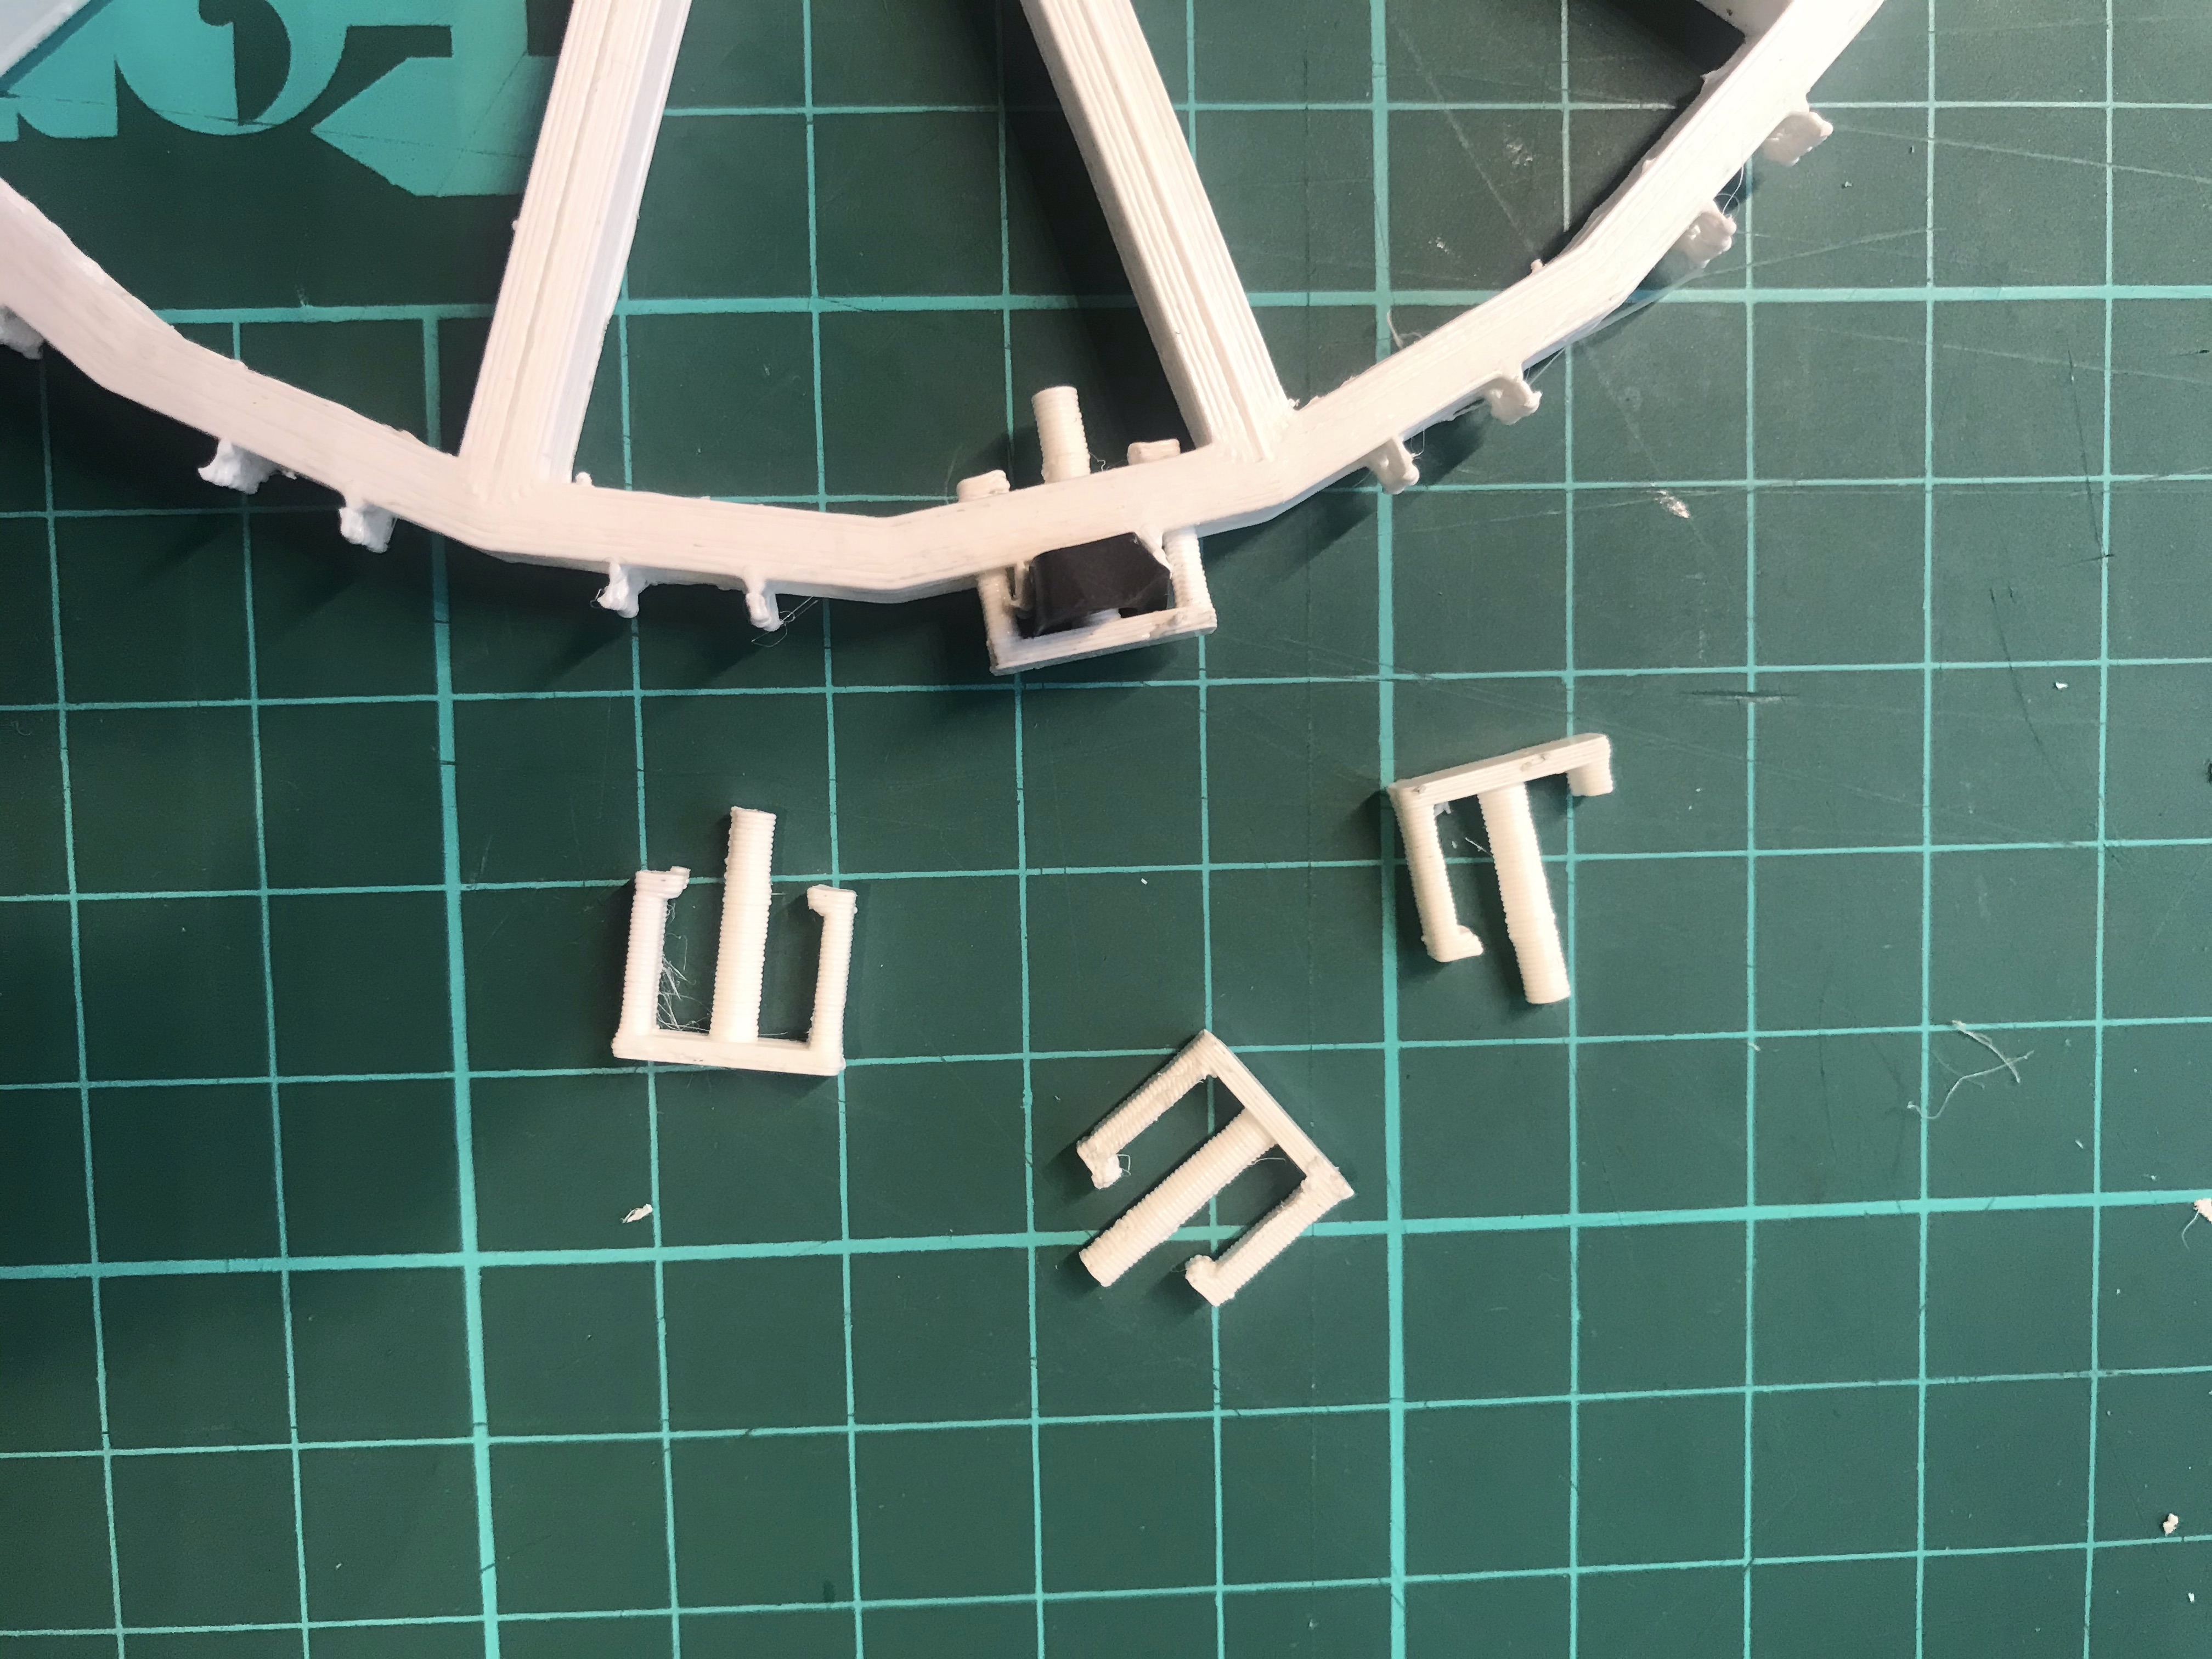
\includegraphics[width=4.166667in, keepaspectratio=true]{./Masterproef_Tool_Wear_Inspection_-_Update_4_DH/voorbeelden van clips op 1cm mat.jpeg}

 

Met vriendelijke groeten,

 

Lars De Pauw



\subsection{Reply}

Hallo Lars,



Ziet er zeer goed uit. Het kan ook helpen om de clips te printen zoals ze nu liggen ipv rechtopstaand. Als je wil bestel ik printmateriaal voor u. Zou het beter zijn om PETG te gebruiken voor de sterkte? Ik zal ook een aantal aluminium profielen bestellen waarmee je gemakkelijk een constructie kan maken om de camera aan te bevestigen.



Stuur me anders je adres door dan laat ik het meteen bij jou leveren.



Mvg,



\subsection{Mail}

Beste meneer Hulens,

 

De clips liggend printen zou zeker helpen voor de sterkte, maar dat zorgde er voor dat de vorm van de middelste pin niet volledig rond was. Gezien deze pin door het gat in de plaatjes moet is het hier wel belangrijk dat deze mooi rond is.

 

PETG lijkt hier inderdaad een betere optie dan ABS, die mag u zeker bestellen en laten leveren net als de aluminium profielen.

 

Het leveradres is dan:



 

Alvast bedankt!

Met vriendelijke groeten,

 

Lars De Pauw



\end{document}
